\documentclass[conference]{IEEEtran}
\IEEEoverridecommandlockouts
% The preceding line is only needed to identify funding in the first footnote. If that is unneeded, please comment it out.
\usepackage{cite}
\usepackage{amsmath,amssymb,amsfonts}
\usepackage{algorithmic}
\usepackage{graphicx}
\usepackage{textcomp}
\usepackage{xcolor}
\usepackage{subfigure}
\usepackage{cases}
\def\BibTeX{{\rm B\kern-.05em{\sc i\kern-.025em b}\kern-.08em
    T\kern-.1667em\lower.7ex\hbox{E}\kern-.125emX}}
\begin{document}

\title{Chaos-based Steganography for Medical Images\\
{\footnotesize \textsuperscript{*}Note: Sub-titles are not captured in Xplore and
should not be used}
\thanks{Identify applicable funding agency here. If none, delete this.}
}

\author{\IEEEauthorblockN{1\textsuperscript{st} Given Name Surname}
\IEEEauthorblockA{\textit{dept. name of organization (of Aff.)} \\
\textit{name of organization (of Aff.)}\\
City, Country \\
email address or ORCID}
\and
\IEEEauthorblockN{2\textsuperscript{nd} Given Name Surname}
\IEEEauthorblockA{\textit{dept. name of organization (of Aff.)} \\
\textit{name of organization (of Aff.)}\\
City, Country \\
email address or ORCID}
\and
\IEEEauthorblockN{3\textsuperscript{rd} Given Name Surname}
\IEEEauthorblockA{\textit{dept. name of organization (of Aff.)} \\
\textit{name of organization (of Aff.)}\\
City, Country \\
email address or ORCID}
\and
\IEEEauthorblockN{4\textsuperscript{th} Given Name Surname}
\IEEEauthorblockA{\textit{dept. name of organization (of Aff.)} \\
\textit{name of organization (of Aff.)}\\
City, Country \\
email address or ORCID}
\and
\IEEEauthorblockN{5\textsuperscript{th} Given Name Surname}
\IEEEauthorblockA{\textit{dept. name of organization (of Aff.)} \\
\textit{name of organization (of Aff.)}\\
City, Country \\
email address or ORCID}
\and
\IEEEauthorblockN{6\textsuperscript{th} Given Name Surname}
\IEEEauthorblockA{\textit{dept. name of organization (of Aff.)} \\
\textit{name of organization (of Aff.)}\\
City, Country \\
email address or ORCID}
}

\maketitle

\begin{abstract}
This document is a model and instructions for \LaTeX.
This and the IEEEtran.cls file define the components of your paper [title, text, heads, etc.]. *CRITICAL: Do Not Use Symbols, Special Characters, Footnotes, 
or Math in Paper Title or Abstract.
\end{abstract}

\begin{IEEEkeywords}
component, formatting, style, styling, insert
\end{IEEEkeywords}

\section{Introduction}

\section{Steganographic techniques}\label{steTechniques}
Steganography has a long history of been used as a way to protect security and privacy of valuable information. While cryptography focuses on protecting the secret message by jumbling its content, steganography concerns on protecting the secret message by concealing its mere existence. The concealment of secret messages is achieved by embedding them into other seemingly-innocent host mediums. Depend on the type of the cover object there are many suitable steganographic techniques which are followed in order to obtain security. Taking the cover object as medical image in hiding information is known as image steganography. Generally, in this technique pixel intensities are used to hide the information. Image steganography terminologies are as follows:
\begin{figure}[h!]
	\centering
	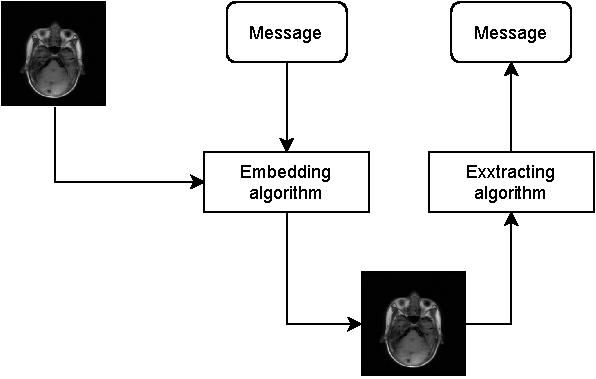
\includegraphics[width=3in]{steganoImage}
	\caption{Steganography in medical images.}\label{fig:steganoImage}
\end{figure}
\begin{itemize}
	\item \indent \textbf{Cover-image:} Original image which is used as a carrier for hidden information.
	\item \indent \textbf{Message:} Actual information which is used to hide into images. Message could be a plain text, a cipher text or some other image.
	\item \indent \textbf{Stego-image:} After embedding message into cover image is known as stego-image.
	\item \indent \textbf{Stego-key (optional):} A key is used for embedding or extracting the messages from cover-images and stego-images.
\end{itemize}
\indent Image steganography shown in Figure~\ref{fig:steganoImage} is the method of information hiding into cover-image and  generates a stego-image and is currently ubiquitous in a great deal of fields such as secure data communication, healthcare and military. \\[0.2cm]
\indent Image steganography techniques can be divided into following domains: spatial domain method, transform domain technique, distortion techniques, masking and filtering. 

\subsection{Spatial Domain Methods}
There are many versions of spatial steganography, all directly change some bits in the image pixel values in hiding data. Least significant bit (LSB)-based steganography is one of the simplest techniques that hides a secret message in the LSBs of pixel values without introducing many perceptible distortions. Changes in the value of the LSB are imperceptible for human eyes. Spatial domain techniques are remarkable such as least significant bit (LSB), pixel value differencing (PVD), edges based data embedding method (EBE), random pixel embedding method (RPE), etc. 

\subsection{Transform Domain Techniques}
This is a more complex way of hiding information in an image because various algorithms and transformations are used on the image to hide information in it. By contrast, the process of embedding data in the frequency domain of a signal is much stronger than embedding principles that operate in the time domain. Most of the strong steganographic systems today operate within the transform domain due to an advantage over spatial domain techniques which is the ability to hide information in areas of the image that are less exposed to compression, cropping, and image processing. Transform domain techniques are broadly declared into: Discrete Fourier transformation technique (DFT), Discrete cosine transformation technique (DCT), Discrete Wavelet transformation technique (DWT), Lossless or reversible method (DCT) and embedding in coefficient bits. 

\subsection{Distortion Techniques}
These techniques need knowledge of the original cover image during the decoding process where the decoder functions to check for differences between the original cover image and the distorted cover image in order to restore the secret  message. The encoder adds a sequence of changes to the cover image. So, information is  described as being stored by signal distortion \cite{b2}. However, the need for sending the cover image limits the benefits of this technique. In any steganographic technique, the cover image should never be used more than once. If an attacker tampers with the stego-image by cropping, scaling or rotating, the receiver can easily detect it. In some cases, if the message is encoded with error correcting information, the change can even be reversed and the original message can be recovered [3].

\subsection{Masking and Filtering}
By marking an image, in the same way as to paper watermarks, these techniques embed the information in more significant areas than just hiding it into the noise level. The hidden message is more integral to the cover image. Watermarking techniques can be applied without the fear of image destruction due to lossy compression as they are more integrated into the image. This method is much more robust than LSB replacement with respect to compression since the information is hidden in the visible parts of the image but there is a limitation in the capacity when techniques can be applied only to gray scale images and restricted to 24 bits. \\
	
\indent Many Steganography schemes for images are proposed. However, the best self-evident and furthermore the most surely understood method for concealing data in pictures is the least significant bit insertion technique in which only the LSB bit planes are replaced with the secret data \cite{b1}. Due to the simplicity of the LSB Steganography scheme it is very easy to detect the data by attackers. It is because of payload embedding which is common for all pixels. To overcome the problem many different techniques have been proposed where the payload is different for each pixels and the bit replaced positions also have changed. Some methods basing on LSB bit planes used for both gray scale and color images are introduced in the next section. To achieve better visual quality of stego-image it takes care of noise sensitive area for embedding basing chaotic functions like logistic map, cat map, standard map. The strength of proposed method is its integrity of secret hidden information in stego-image and high hidden capacity. These methods are also targeted to achieve high hidden capacity plus security of hidden message.  

\section{Chaos-based Steganography schemes}
In this section, we compare a variety of schemes that employs noisy regions in eventual bit-planes (LSBs) of an digital image to hide secret bits to improve the visual quality of stego-images and the security of the hidden data. Message is extracted from the patient information in the medical image respectively and then encrypted using an encryption algorithm. \\[0.2cm]
\indent We consider the mathematical form of a chaotic map in which chaos means a state of disorder. In mathematics, map is an evolution function that shows some sort of chaotic behavior \cite{b4}. A discrete time dynamical system is also called map. Chaotic map has some inherent features \cite{b5} such as:
\begin{itemize}
	\item Sensitive to initial conditions (also called butterfly effect) which means a small modification in initial conditions should produce high deviations of the corresponding output.
	\item Ergodicity implies the output has the	same distribution for any input.
	\item Deterministic means a deterministic process can cause a pseudo-random behavior.
	\item Structure complexity signifies a simple mathematical function has very high complexity.
\end{itemize}
\begin{figure}[h!]
	\centering
	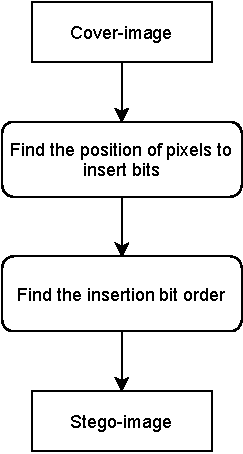
\includegraphics[width=2in,height=3in]{./process}
	\caption{The process of scheme steganography.}\label{fig:process}
\end{figure}
The process of embedding the message in an digital medical image, which is known as the cover-image, is shown in Figure~\ref{fig:process}. We will apply the dynamic functions to determine the appropriate bit insertion positions and the arrangement of the inserted bits in the image. The message is represented in binary format and each group of 2 bit is used to replace 2-LSB of the chosen pixels (2 bit per pixels). In the image extraction phase, we only need to reuse the chaotic maps to calculate the positions, which has been added bits following the correct order in the embedding process and then the message and origin image can be restored.

\subsection{Chaos-based Steganography based on logistic map (CSBLM)}
\indent Firstly, the simplest form of chaotic map, which is developed by May \cite{b6} is logistic map described in Equation~\eqref{eq:logisticmap}.
\begin{align}
x_{n} = \alpha.x_{n-1}(1-x_{n-1}),
\label{eq:logisticmap} 
\end{align}
Here \(x_{0}\) is initial value and n value denotes the number of rounds. 1D logistic map generate chaotic sequences only of the \(\alpha\) value must be in the range of \(3.5 \leq \alpha \leq 4\)\cite{b7}. It produces chaotic sequences within the range [0, 1]. By using these chaotic sequence only, the position of pixels in the cover image are chosen for embedding the bits of the message. \\
\indent In CSBLM, we use the logistic map to make out the inserted pixel positions. The embedding implementation starts with choosing the initial value, system parameter value and iteration value of 1D logistic map such as \(x_{0}\), \(\alpha\) and \(r_{p}\), respectively to generate the chaotic sequence. \[X = \left\{x_{1}, x_{2}, x_{3}, ..., x_{n},\right\}\] where n is the result of multiplying the two-sided dimensions of the cover image. Then, the generated chaotic sequence X is sorted as follows: \[\left[sx_{i}, ax_{i}\right] = sort(X_{i}), i = 1,2,3,...,N,\] where \(sx\) is a new sorted sequence of X, \(ax\) is a new index value of the series X. A group of consecutive 2-bit extracted from the message could replace bits in the 1st and 2nd bit plane corresponding position \(ax_{i}\). Algorithm for embedding process is described as follows: \\[0.2cm]
\textbf{For i = 1 : len / 2} \\
\indent \indent BP(1, M x N) = Replaced 2-LSB of cover image BP(1, \(ax_{i}\)) into G (i); \\
\indent \indent // BP: 2-LSB of cover image\\
\indent \indent // G: groups of two bit\\
\textbf{End}

\subsection{Chaos-based Steganography based on cat map (CSBCM)}
\indent We consider the mathematical form of a 2D chaotic map \(f : S^{2} \rightarrow S^{2}\). This map is described by the following equation:
\begin{align}
(x_{i+1}, y_{i+1}) = f(x_{i}, y_{i}),
\label{eq:2dchaoticmap} 
\end{align}
where \((x_{i}, y_{i})\) and \((x_{i+1}, y_{i+1})\) are the old and new states, respectively. There are a number of different chaotic maps which seem to be suitable for ciphering purposes. However, the only maps of interest are those which are simple so that the ciphering/deciphering phases can be performed quickly. In fact, the maps used in the chaos-based cryptosystem include: Henon map, Lozi map, Duffiggs map, Cat map, Baker map and Standard map. As compared in \cite{b8}, the 2D Cat map has good statistical characteristics and the highest performance. Figure~\ref{fig:Catmap} describes the scheme of the proposed embedding process in medical images based on the 2D Cat map, which represents a nonlinear embedding algorithm.
\begin{figure}[h!]
	\centering
	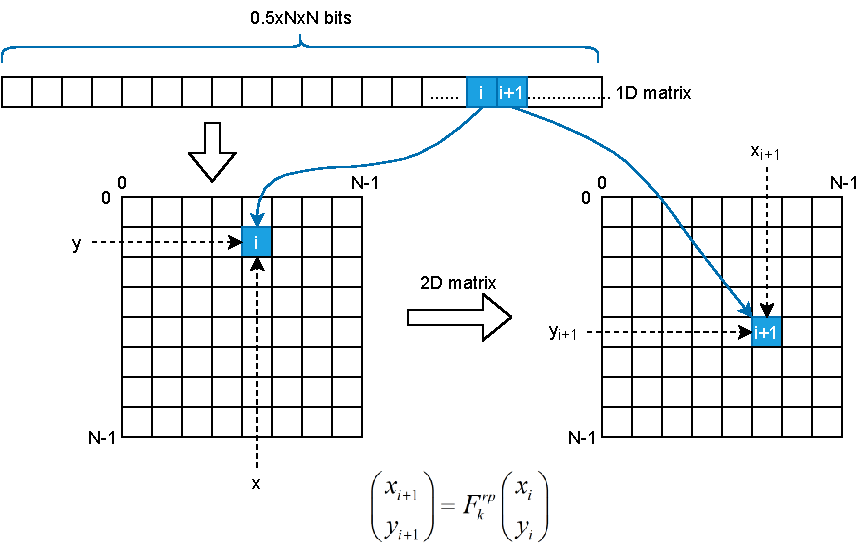
\includegraphics[width=0.45\textwidth]{./Catmap}
	\caption{The scheme steganography base on the Cat map.}\label{fig:Catmap}
\end{figure}
The new bit's position is calculated as follows function~\ref{eq:2dchaoticmap}. Here, \(F: [0,N - 1]^{2} \rightarrow [0,N - 1]^{2}\) is the discrete Cat map defined as:
\begin{subnumcases}{}
x_{i+1} = mod(x_{i} + a \times y_{i}, 1)\notag$$ \\  
y_{i+1} = mod(b \times x_{i} + a \times b \times y_{i}, 1)\notag$$
\label{eq:2dchaoticmap}
\end{subnumcases} \\
DATA EMBEDDING PHASE \\[0.2cm]
\indent In the embedding process the medical image and the message which is encrypted in the pre-process and is converted to the binary format are completely selected. We make use of cat map function with an appropriate set of initialization values and a proper iteration number to calculate two coordinates of the pixel location which is used to insert bits. Similar to the previous method, we perform respectively 2-bit substitution at position coordinates have been determined without changing bit planes into 1D-array as using the logistic map. \\[0.2cm]
DATA EXTRACTION PHASE \\[0.2cm]
\indent The secret message from the stego image can be retrieved only by using the extracting algorithm by using the same initial values and Cat map function. The inserted pixel location is calculated again by using 2-dimensions map corresponding. This algorithm provides extreme sensitivity as well as security. 

\subsection{Chaos-based Steganography based on mixing 1D and 2D chaotic maps (CSBMM)}
\indent Last but not least, the approach is the likelihood to consolidate the strategies of information hiding by using both the 1-dimension an 2-dimension function which are known as logistic map and cat map, correspondingly. The later is used to find the pixel position to insert bits and the former plays an important role in deciding the order of the replaced bits. \\
\indent Comparing with two methods above, after using the 2D chaotic map, namely the cat map, we must put adopted pixels in a one-dimension sequence instead of having to perform bit insertion directly in these pixels. Moreover, there is a significant change between CSBMM and the previous methods when 2-LSB bits are not replaced by two consecutive bits extracted from the message because the sorting order of set bits is decided by the logistic map. 

\section{EXPERIMENTAL RESULTS AND COMPARISIONS}
\indent In this section, several experiments are carried out on the set of selected grey and color images to hide an encrypted message with the proposed LSB methods. The factors to be considered while designing a steganography system are:
\begin{enumerate}
	\item Number of bits to be embedded (capacity).
	\item Visual quality of the image.
	\item Less distortion in the embedded cover image compared to original image.
	\item Level of security.
\end{enumerate}
The performance is evaluated based on PSNR (Peak Signal to Noise Ratio) which defines the quality of the image. The PSNR is defined as follows
\begin{align}
PSNR = 10log_{10}(\frac{255^{2}}{MSE}) (dB)
\label{eq:psnr} 
\end{align}
where MSE is Mean Square Error between the original image and the stego image. The MSE is defined as follows.
\begin{align}
MSE = \frac{1}{M \times N}\sum_{i = 0}^{M - 1}\sum_{j = 0}^{N - 1}(R_{ij} - K_{ij})^{2}
\label{eq:mse} 
\end{align}
where \(R_{ij}\) and \(K_{ij}\) are pixel values of the original image and the stego-image. \(M \times N\) represents all the pixel values of the image. Larger the PSNR and smaller the MSE values better the quality which means the stego-image will be almost similar to the original image. \\
\indent wPSNR \cite{b9} is currently the most commonly used metric for embedding quality. It is well known that PSNR does not calculate the stego-image quality well. wPSNR is a more accurate metric, because it considers the texture masking effect. wPSNR is more accurare in spatial domain and is not a feasible metric in frequency domain embedding. Texture masking
effect or noise visibility function (NVF) is the increasing of imperceptibility of noise-like secure data because of the existence of a similar noisy-effect in the cover image. In
general, the secure data embedding is difficult to be noticed in the texture regions. wPSNR is calculated by
\begin{align}
wPSNR = 10log_{10}(\frac{max(I)^{2}}{||NVF(S - I)||^{2}}) (dB)
\label{eq:wPSNR} 
\end{align}
where I and S are the cover and stego-images. \\[0.2cm]

\begin{table*}[htbp]
	\caption{Characteristics of various steganography algorithms used in medical images}
	\centering
		\begin{tabular}{ |c|c|c|c|c|c|c|c|c|c|c|c|c| }
			\hline
			\textbf{Image}&\multicolumn{4}{|c|}{\textbf{CSBLM}}&\multicolumn{4}{|c|}{\textbf{CSBCM}}&\multicolumn{4}{|c|}{\textbf{CSBMM}}\\
			\cline{2-13}
			\textbf{} & \textbf{\textit{PSNR(dB)}}& \textbf{\textit{wPSNR(dB)}}& \textbf{\textit{MSE}}& \textbf{\textit{SSIM}}& \textbf{\textit{PSNR(dB)}}& \textbf{\textit{wPSNR(dB)}}& \textbf{\textit{MSE}} & \textbf{\textit{SSIM}} & \textbf{\textit{PSNR(dB)}}& \textbf{\textit{wPSNR(dB)}}& \textbf{\textit{MSE}} & \textbf{\textit{SSIM}} \\
			\hline
			(a) & 50.951 & 59.424 & 0.522 & 0.992 & 50.824 & 60.653 & 0.538 & 0.993 & 50.897 & 60.556 &	0.529 & 0.993\\
			(b) & 50.941 & 54.585 &	0.524 & 0.991 & 50.902 & 55.417	& 0.528 & 0.991 & 50.891 & 55.297	& 0.530 & 0.991\\
			(c) & 50.933 & 68.036 &	0.525 & 0.990 & 50.841 & 68.791 &	0.536 & 0.990 & 50.895 & 68.793 &	0.529 & 0.990\\
			(d) & 50.966 & 57.376 &	0.521 & 0.990 & 50.906 & 58.131	& 0.528 & 0.990 & 50.944 & 58.150	& 0.523 & 0.991\\
			(e) & 50.860 & 61.655	& 0.533 & 0.991 & 50.788 & 62.557	& 0.542 & 0.991 & 50.768 & 62.580	& 0.545 & 0.991\\
			\hline
		\end{tabular}
	\label{tab:Characteristics}
\end{table*}
\indent The Structural Similarity Index (SSIM) is a perceptual metric that quantifies image quality degradation. SSIM actually measures the perceptual difference between two similar images. It is a full reference metric that requires two images from the same image capture- a reference image and a processed image but it cannot judge which of the two is better: that must be inferred from knowing which is the “original” and which has been subjected to additional processing such as data compression. The Structural Similarity Index (SSIM) metric extracts 3 key features from an image:
\begin{itemize}
	\item Luminance
	\item Contrast
	\item Structure
\end{itemize}
The system calculates SSIM between 2 given images which is a value between -1 an +1. A value of +1 indicates that the 2 given images are \textbf{very similar or the same} while a value of -1 indicates that are \textbf{very different}. The SSIM score is given by 
\begin{align}
SSIM(x,y) = [\textsl{l}(x,y)]^{\alpha}.[\textsl{c}(x,y)]^{\beta}.[\textsl{s}(x,y)]^{\gamma}
\label{eq:ssim} 
\end{align}
where x and y are two images being compared, \(\alpha > 0, \beta > 0, \gamma > 0\) denote the relative importance of each of the metric and l, c, s are the luminance, contrast and structure comparison function, respectively. \\
\begin{figure}
\centering
\begin{subfigure}[]{}
	\centering
	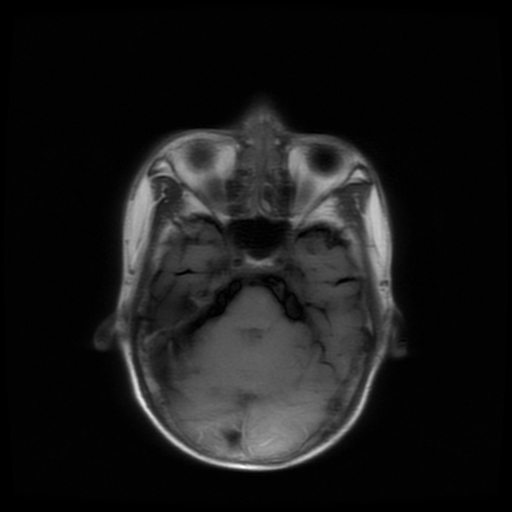
\includegraphics[width=2cm,height=2cm]{./image/IMG-0004-00001}
\end{subfigure}
\begin{subfigure}[]{}
	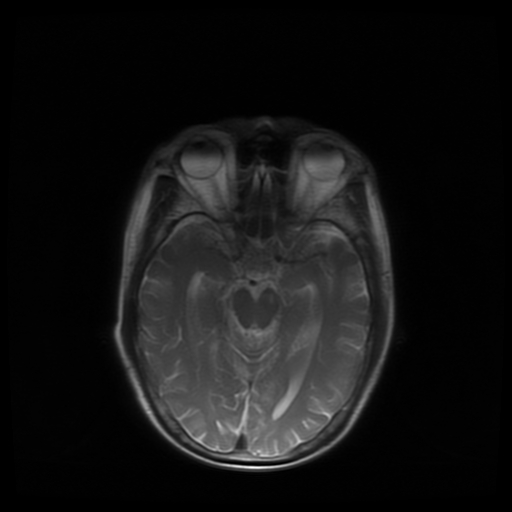
\includegraphics[width=2cm,height=2cm]{./image/IMG-0004-00002}
\end{subfigure}
\begin{subfigure}[]{}
	\centering
	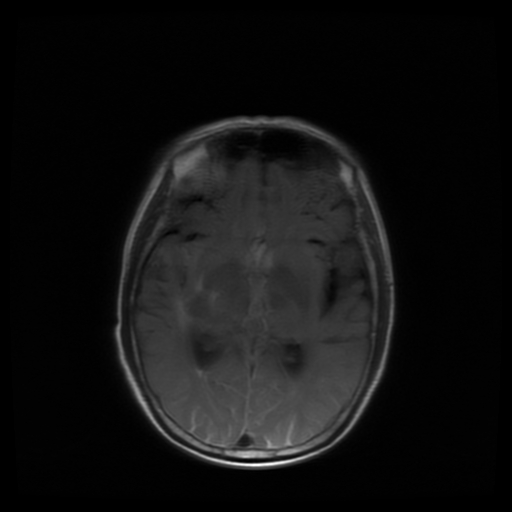
\includegraphics[width=2cm,height=2cm]{./image/IMG-0004-00003}
\end{subfigure}
\\
\begin{subfigure}[]{} 
	\centering
	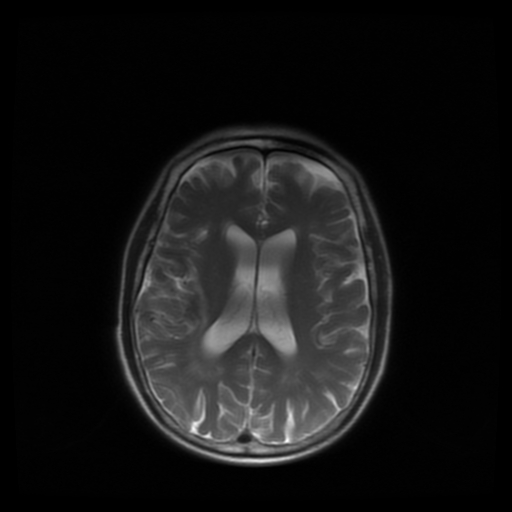
\includegraphics[width=2cm,height=2cm]{./image/IMG-0004-00004}
\end{subfigure}
\begin{subfigure}[]{}
	\centering
	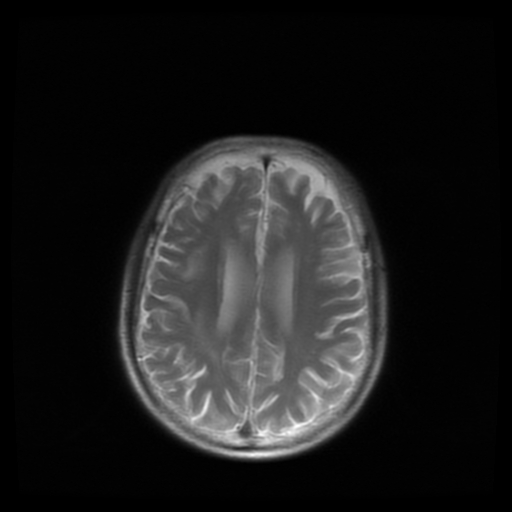
\includegraphics[width=2cm,height=2cm]{./image/IMG-0004-00005}
\end{subfigure}
\caption{Five brain MRI cover images.}
\label{fig:inputImages}
\end{figure}
\indent The code has been executed with a set of test images which include 30 images, for example, as shown in Figure~\ref{fig:inputImages}. The value of variables MSE, PSNR and wPSNR values are shown in the Table~\ref{tab:Characteristics}
\begin{figure}
\subfigure[Cover-image]
  {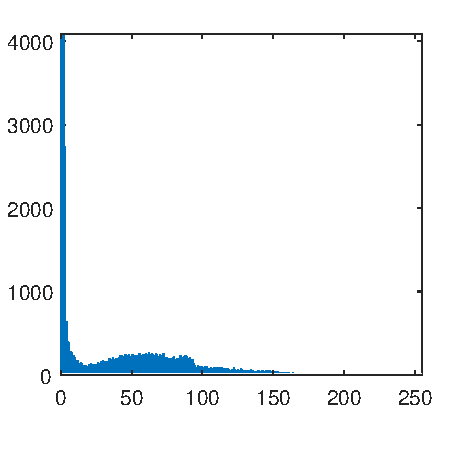
\includegraphics[width=1.5in,height=1in]{histogram1}}\hfill
\subfigure[Stego-image of CSBLM]
  {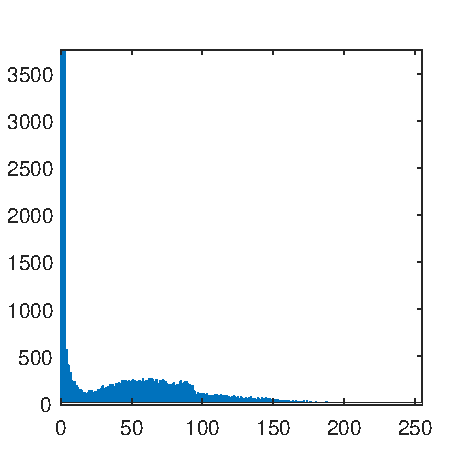
\includegraphics[width=1.5in,height=1in]{histogram2}}\\
\subfigure[Stego-image of CSBCM]
  {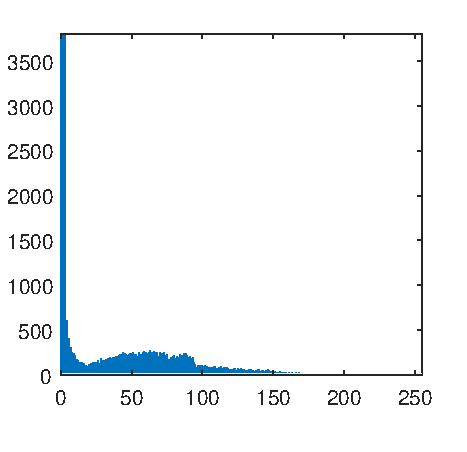
\includegraphics[width=1.5in,height=1in]{histogram3}}\hfill
\subfigure[Stego-image of CSBMM]
  {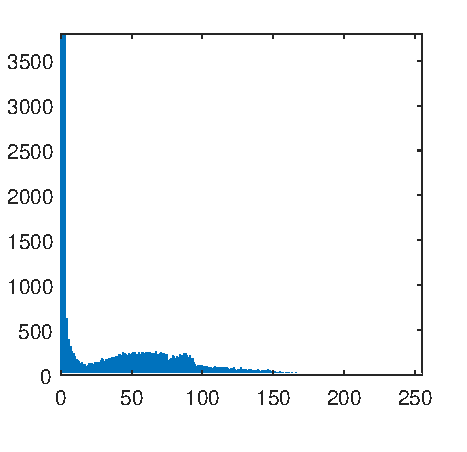
\includegraphics[width=1.5in,height=1in]{histogram4}}\\
\caption{Histogram comparison between the cover-image and three kinds of stego-images}
\label{fig:timecomparison}
\end{figure}

\begin{table}[htbp]
	\caption{The comparison of the image quality rating values and the execution time with payload = \(2^{15}\) bits and iteration \(r_{p}\) = 100 in the same \(256 \times 256\) cover image. }
	\centering
	\begin{tabular}{|c|c|c|c|}
		\hline
		\textbf{Characteristics}&\textbf{CSBLM}&\textbf{CSBCM}&\textbf{CSBMM}\\
		\cline{1-4}
		\hline
		Embedding time (s) & 0.432 & 0.600 & 0.624 \\
		Total time (s) & 0.724 & 1.020 & 1.064 \\
		PSNR (dB) & 50.951 & 50.824 & 50.897 \\
		wPSNR (dB) & 59.424 & 60.653 & 60.556 \\
		MSE & 0.522 & 0.538 & 0.529	\\
		SSIM & 0.992 & 0.993 & 0.993 \\
		\hline
	\end{tabular}
	\label{tab:256256Comparison}
\end{table}

\begin{table}[htbp]
	\caption{The comparison the image quality rating values and the execution time with payload = \(2^{17}\) bits and iteration \(r_{p}\) = 100 in the \(512 \times 512\) cover image. }
	\centering
	\begin{tabular}{|c|c|c|c|}
		\hline
		\textbf{Characteristics}&\textbf{CSBLM}&\textbf{CSBCM}&\textbf{CSBMM}\\
		\cline{1-4}
		\hline
		Embedding time (s) & 1.496 & 2.230 & 2.233 \\
		Total time (s) & 2.509 & 3.892 & 3.918 \\
		PSNR (dB) & 50.737 & 50.721 & 50.733 \\
		wPSNR (dB) & 69.867 & 69.816 & 69.841 \\
		MSE & 0.549 & 0.551 & 0.549	\\
		SSIM & 0.991 & 0.991 & 0.991 \\
		\hline
	\end{tabular}
	\label{tab:512512Comparison}
\end{table}

\begin{figure}
\subfigure[Embedding process]
  {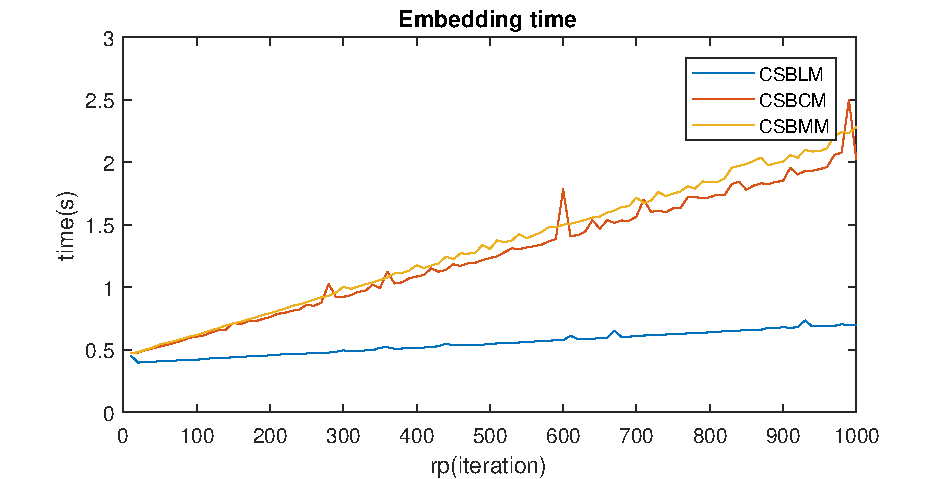
\includegraphics[width=1.5in,height=0.9in]{TimeSpeedEmbedrp10to1000}}\hfill
\subfigure[Embedding and extracting process]
  {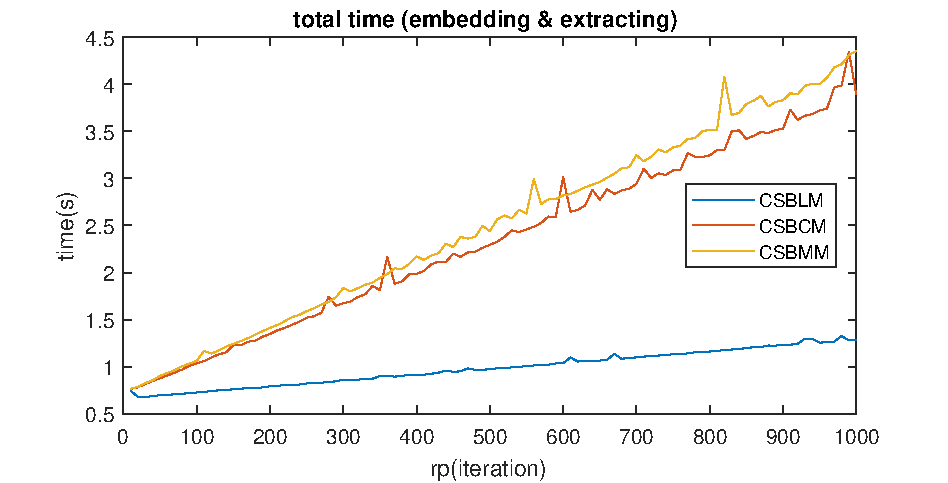
\includegraphics[width=1.5in,height=0.9in]{TimeSpeedTotalrp10to1000}}
\caption{Time speed comparison when the iteration value changes from 10 to 1000.}
\label{fig:timecomparison}
\end{figure}
\begin{figure}
\subfigure[Embedding process]
  {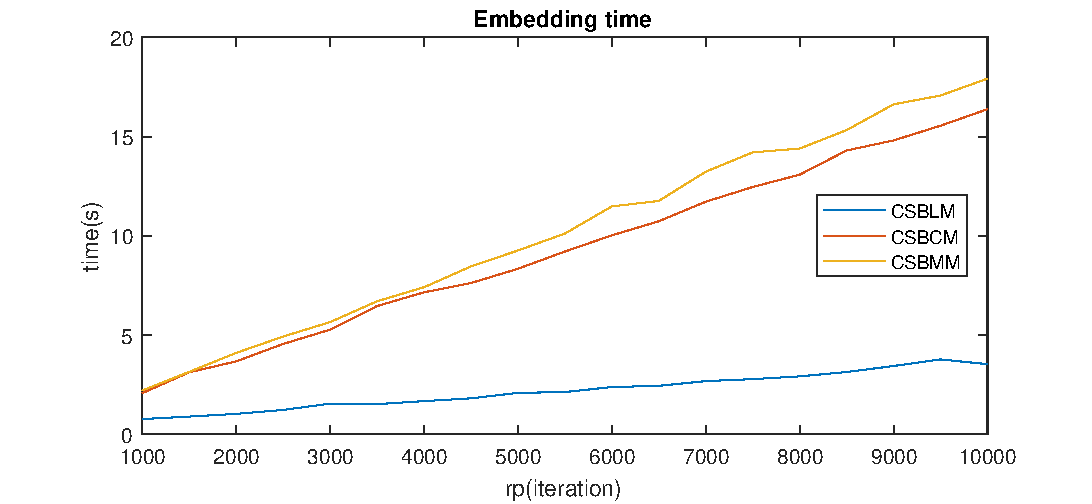
\includegraphics[width=1.5in,height=0.9in]{TimeSpeedEmbedrp1000to10000}}\hfill
\subfigure[Embedding and extracting process]
  {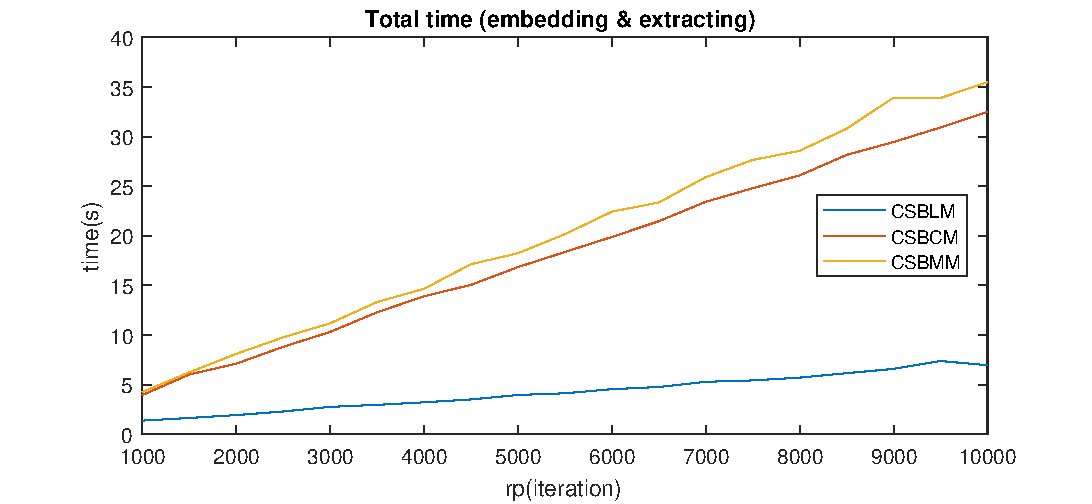
\includegraphics[width=1.5in,height=0.9in]{TimeSpeedTotalrp1000to10000}}
\caption{Time speed comparison when the iteration value changes from 1000 to 10000.}
\label{fig:timecomparison}
\end{figure}

\section*{Acknowledgment}

The preferred spelling of the word ``acknowledgment'' in America is without 
an ``e'' after the ``g''. Avoid the stilted expression ``one of us (R. B. 
G.) thanks $\ldots$''. Instead, try ``R. B. G. thanks$\ldots$''. Put sponsor 
acknowledgments in the unnumbered footnote on the first page.

\begin{thebibliography}{00}
\bibitem{b1} C.C.  Chang,  M.H.  Lin,  and  Y.C.  Hu  ,  “A  fast  and  secure  image hiding scheme based on LSB substitution,” International journal of pattern  recognition  and  artificial    intelligence,  vol.  16,  no.  4,  pp. 399–418, June 2002.
\bibitem{b2} H.S. Majunatha Reddy and K.B. Raja. (2009). High capacity and security steganography using discrete wavelet transform.  International Journal of Computer Science and Security. pp. 462-472.
\bibitem{b3} P. Kruus, C. Scace,M. Heyman, and M. Mundy., A survey of steganography techniques for image files . Advanced Security Research Journal. [On line], 5(1), (2003), pp. 41-52. 
\bibitem{b4} M. Fran¸cois, T. Grosges, D. Barchiesi, and R. Erra, "Pseudo-random number generator based on mixing of three chaotic maps," Communications in Nonlinear Science and Numerical Simulation, vol. 19, no. 4, pp. 887-895, 2014.
\bibitem{b5} Z. Liu and L. Xi, "Image information hiding encryption using chaotic sequence," in International Conference on Knowledge-Based and Intelligent Information and Engineering Systems, pp. 202-208, Springer, 2007.
\bibitem{b6} R. M. May, et al., "Simple mathematical models with very complicated dynamics," Nature, vol. 261, no. 5560, pp. 459-467, 1976.
\bibitem{b7} X. Wang, J. Zhao, and H. Liu, "A new image encryption algorithm based on chaos," Optics Communications, vol. 285, no. 5, pp. 562-566, 2012.
\bibitem{b8} Mrs Hue.
\bibitem{b9} Voloshynovskiy S et al. Generalized watermarking attack based on watermark estimation and perceptual remodulation. in Proceeding of Electronic Imaging. International Society for Optics and Photonics, 2000; 358-370.
\end{thebibliography}

\end{document}
